\documentclass[letterpaper]{article}

\usepackage[english]{babel}
\usepackage[utf8x]{inputenc}
\usepackage{amsmath}
\usepackage{amsfonts}
\usepackage{amssymb}
\usepackage{mathtools}
\usepackage{graphicx}
\usepackage{xcolor}

\usepackage[top=1.3in, bottom=1.5in, left=1in, right=1in]{geometry}
\usepackage{fancyhdr}
\usepackage{lastpage}
\usepackage{caption}
\usepackage{subcaption}
\usepackage{float} % Use [H] to force figure placement

\usepackage{algorithm}
\usepackage{algpseudocode}
\usepackage[style=alphabetic]{biblatex}

\addbibresource{bib.bib}

\newcommand{\Problem}{C}
\newcommand{\Team}{2126824}

% If you're new to latex, pagewrapping will be your enemy, both in terms of getting floating images/tables to appear on the correct page, and in terms of attractive text line breaking.
% Two tips to help deal with this:
%   - The ``float'' package above allows you to use the [H] option on figures, which forces them to appear in EXACTLY that spot in the docutment. This can be useful to tune things by hand
%   - If latex wants to break apart your text in an awkward way, try wrapping it in a minipage environment. This especially useful for keeping bulleted lists together, as latex often likes to break them across pages.


% Make the bulleted lists use dashes
\renewcommand{\labelitemi}{\normalfont\bfseries\textendash}

\DeclareMathOperator*{\argmin}{arg\,min}

\title{Analyzing Reporting Sightings of Vespa Mandarina}

\author{}
\date{\today}

\begin{document}


% Set up the header and footer
\pagestyle{fancy}
\lhead{2126824}
\rhead{ Page \thepage\ of \pageref{LastPage}}
\rfoot{}    
\cfoot{}
\lfoot{}
\fancypagestyle{plain}{
  \lhead{2126824}
  \rhead{ Page \thepage\ of \pageref{LastPage}}
  \rfoot{}    
  \cfoot{}
  \lfoot{}
}

\renewcommand{\headrulewidth}{0.4pt}
\renewcommand{\footrulewidth}{0.0pt}
%\headrulewidth 0.4pt
%\footrulewidth 0 pt

\graphicspath{{.}}  % Place your graphic files in the same directory as your main document
\DeclareGraphicsExtensions{.pdf, .jpg, .tif, .png}
\thispagestyle{empty}
\vspace*{-16ex}
\centerline{\begin{tabular}{*3{c}}
	\parbox[t]{0.3\linewidth}{\begin{center}\textbf{Problem Chosen}\\ \Large \textcolor{red}{\Problem}\end{center}}
	& \parbox[t]{0.3\linewidth}{\begin{center}\textbf{2021\\ MCM/ICM\\ Summary Sheet}\end{center}}
	& \parbox[t]{0.3\linewidth}{\begin{center}\textbf{Team Control Number}\\ \Large \textcolor{red}{\Team}\end{center}}	\\
	\hline
\end{tabular}}

Our neural network determined that the unidentified wasp with the 
\textbf{global ID} = \textbf{\{1E2B3656-E2CD-4DA9-8CEF-FDE70664643B\}} was a Vespa mandarinia hornet. Unfortunately the accuracy of the statement is very questionable with only \textbf{65.6\%} accuracy, so there is a very real chance we missed one or two hornets. There could potentially be trained a more accurate algorithm through mirroring techniques and using previously trained neural networks, but it is unlikely a high accuracy can be reached with so little confirmed positive cases.

Thankfully, the general location of positively identified hornets makes for an elementary decision where to allocate resources, as all the confirmed cases have been in the North-Western part of Washington near Vancouver in port cities. Climate patterns demonstrate that only the coastal area will really be able to sustain the wasps so state government resources can be focused there.

We managed to generate three models using the provided data to various degrees of success. The most successful one looked at the latitude and longitude in order to predict where wasps would be without any more information that'd improve the accuracy such as elevation or population density. The second most successful model was a neural network that predicted whether something was a wasp based on the images fed into it that was slightly less accurate. The worst of the bunch was a frequency analysis model that looked at the notes sent in by people to try and predict whether something was a wasp, and it ended up being the least accurate of the bunch, demonstrating that citizenry should not be allowed to determine whether something is a Vespa mandarinia hornet or not.

Afterwards we used the latitude-longitude model in order to see if we could find any additional wasps from the unverified data and found the aforementioned one. As more data comes in over time, particularly more positive matches, we will be able to more accurately determine whether a wasp is the desired hornet through the image and lat/lon algorithms. 

It can be pretty easily determined when the pest is eliminated when there are no new cases of the hornet turning up in North Western Washington following several additions to the dataset for positive matches in order to increase the accuracy of the models. However, in absence of a more highly trained model with a bigger training set for Positive ID's, further investigation into the hornet population will require further lab analysis and verification of reports. 

\printbibliography

\pagebreak
\tableofcontents
\pagebreak

\section{Introduction}

Following the discovery and destruction of a Vespa mandarinia hornet nest there have been multiple sightings of this largest wasp in the world. Even at small numbers they are capable of destroying colonies of bees at brutal efficiency, so it is crucial that the spread of these wasps is curbed and eradicated. Throughout this report we will be looking at three different models looking at different parts of the given dataset as well as an exploratory data analysis of the whole scenario to see how the models will stack up with common sense. 


\section{Problem Statement}
We are asked to determine whether the spread of Asian Giant Hornets can be predicted using the given data. Furthermore, we asked to identify mistaken classifications and develop a model by which reports can be prioritized. Finally, we must consider how our model can be updated with new reports over time, and how we can use our model to identify when the hornet have been eliminated. 

\subsection{Problem Assumptions}

We are only given the latitude and longitude, so we are making several assumptions from that. The biggest is that we assume that the entire state of Washington is flat, since there'll be no difference in latitude and longitude whether the overall distance is going through the mountains or over a flat plain. The same can be said of other terrain types, the dataset completely ignores it, which can be relevant between populated and more wooded/wild regions of Washington where the hornet cannot be found as easily. 

A secondary assumption was made for the frequency analysis model, where we made the assumption that people were intelligent actors off whose statements we can determine if an observation contained the hornet or not. We were wrong.

\section{Background}
Vespa Mandarina, commonly referred to as Asian Giant Hornets, sparrow wasps, and “killer hornets”, are a species of large hornet most commonly found in Japan [\cite{penn}]. With recent confirmed sightings on Vancouver Island and in Washington States, there has been growing public alarm about a larger scale invasion of the western North America region. This alarm is indeed justified, as Asian Hornets have demonstrated themselves to be dominating invasive species, under certain circumstances. One of the key attributes that allows hornets to be so easily invasive is their adaptability to new environments due to their eusocial behavior –– however, in new environments hornet species will often lose their eusocial behavior and live as ‘rogue’ wasps. Without the power of eusocial behavior, Asian hornets lose their ability to reproduce at high rates, thus decreasing their overall population – furthermore, they lose their ability to swarm beehives, although they will still pick off individual bees. According to \cite{french}, only 9 out of 34 introductions of the species to new environments have created an invasive species issue – but it is important to note that most of these introductions have been in Europe, and whether the species becomes invasive is depend on environment in which the hornets find themselves and the susceptibility of native species to lose resources or members to the hornets. Of particular susceptibility to the hornets are honeybees, causing a rising concern amongst beekeepers and the creation of a hive attack hotline in Washington State. While bees in Japan have had ample opportunity to adapt, going as far as to even develop specific tactical response to hornets (\cite{french}), this response is not present in honeybees cultivated in America, who are further rendered defenseless by the Asian Hornet’s immunity to bee stings. 

The dangers of an expanding Asian Hornet population in North America include economic impact to beekeepers, who may have to invest in hornet management or relocate (\cite{niche}), human danger from the highly venomous stings, environmental impact of their presence and the subsequent elimination of invasive species, and further expansions into other areas. With regard to further expansion, it should be noted that V. mandarina has a tendency to relocate by hibernating or building nests in shipping containers (\cite{niche}), of which there are plenty in region, with 75 shipping ports in Washington State alone. This could lead to reintroduction of the species even after elimination, and could also result in spread to other areas across the world. Furthermore, while there is no evidence of Asian hornets in eastern America, \cite{niche} warns that areas across North America (as well as parts of South America, central Africa, eastern Australia, and New Zealand) have highly suitable climates for the Asian Hornets to thrive.

\section{Data Sources}
\subsection{Provided Data}
The data set provided consisted of $4,440$ reported sightings by the public. Each report contains the following fields:


\begin{itemize}
    \item GlobalID: unique identifier for the report
    \item Detection Date: date of sighting 
    \item Notes: description of observation from the reporter
    \item Lab Status: Takes one of 4 possible values
    \begin{itemize}
        \item Positive ID: Indicates the report has been verified by the lab
        \item Negative ID: Indicates the lab has confirmed the report to be false
        \item Unverified: Indicates no determination could be made by the lab regarding the validity of the report, due to lack of information
        \item Unprocessed: Indicates the sighting has not yet been classified
    \end{itemize}
    \item Lab Comments: information added to the lab after investigation
    \item Submission Date: date report was submitted
    \item Latitude Coordinate
    \item Longitude Coordinate
    
\end{itemize}


\begin{flushleft}
Also provided are pictures of reported sightings, when submitted by the reporter.

Our first step in analyzing the data is to sort it by Lab Status to provide insight regarding the distribution of the data and to allow us to identify factors that lead to reports being placed in each category. The vast majority of data points fall into the Negative ID or Unverified category (47\% and 53\%, respectively), while a much smaller portion - $.32\%$ - are categorized as Positive ID's.

\end{flushleft}

\begin{center}
\captionof{table}{} \label{tab:title} 
 \begin{tabular}{||c c c c c||} 
 \hline
 \multicolumn{5}{|c|}{Distribution of Data by ID Type} \\
 \hline
 Category & Positive ID & Negative ID & Unverified & Unprocessed  \\ [0.5ex] 
 \hline
 Number of Reports & 14 & 2069 & 2342 & 15 \\ 
 \hline
\% of Reports & .3182\% & 47.0227\% & 53.2273\% & .3409\% \\

 \hline
\end{tabular}

\end{center}

\begin{flushleft}
In order to discover trends in the data points over time, we then sorted the data in each ID group by Detection Date. In the process of sorting by time, several reports with no Detection Date were identified; others had impossible Detection Dates, such as June 21st of the year 515.To ascertain how much data was invalid in this way, we analyzed the number of the reports, by category, before specified years (Table 2). 
\end{flushleft}

\begin{center}
\captionof{table}{} \label{tab:title} 
 \begin{tabular}{||c c c c c||} 
 \hline
 \multicolumn{5}{|c|}{Distribution of Data by Detection Date and ID Type} \\
 \hline
 Category & Positive ID & Negative ID & Unverified & Unprocessed  \\ [0.5ex] 
 \hline
 \# of Reports Before 1980 & 0 (0\%) & 1 (.0483\%) & 10 (.4270\%) & 0 (0\%) \\ 
 \hline
\# of Reports Before 2000 & 0 (0\%) & 1 (.0483\%) & 11 (.4697\%) & 0 (0\%) \\
\hline
\# of Reports Before 2010 & 0 (0\%) & 1 (.0483\%) & 12 (.5124\%) & 0 (0\%) \\
\hline
\# of Reports Before Sep, 2019 & 0 (0\%) & 35 (1.6916\%) & 131 (5.5935\%) & 2 (13.3333\%) \\
\hline
Range of Dates & 2019 - 2020 & 1200 - 2020 & 515 - 2020 & 2015 - 2020 \\
\hline
\end{tabular}
\end{center}


\begin{figure}[H]
\centering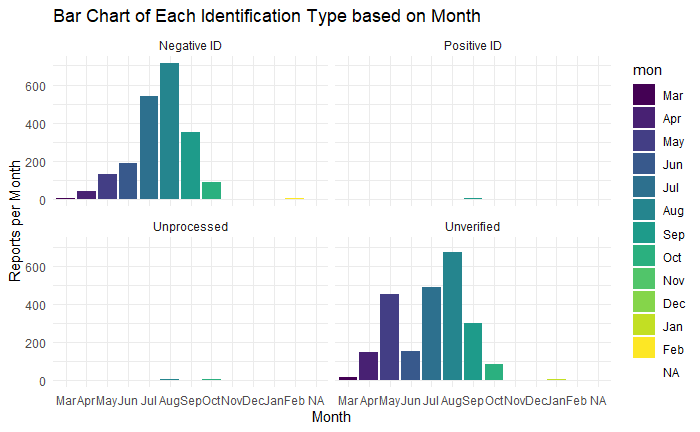
\includegraphics[height = 7cm]{compareDistributions.png}
\caption{Distribution of Reports By Month}
\end{figure}
There does not appear to be significant variation in the distribution of reports over time for each of the four the positive and negative ID categories, reflecting that date of submission will likely not be a contributing factor for a model to predict the classification of reports.



\begin{figure}[H]
\centering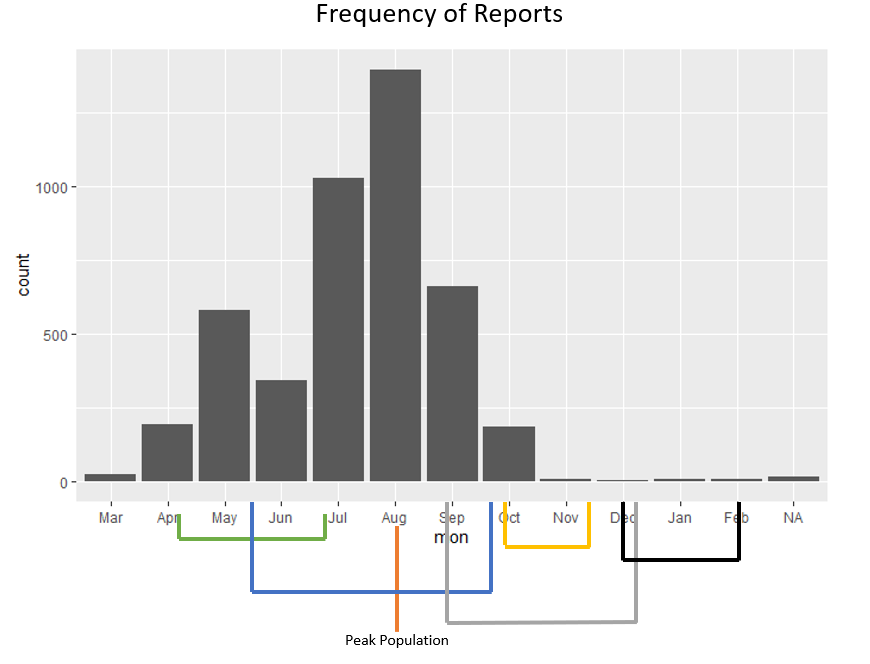
\includegraphics[height = 7cm]{frequencies_yeehaw.PNG}
\caption{Distribution of Reports Against Colony Cycle}
\end{figure}
We also set out to ascertain whether the data we are presented with is reasonable - i.e., are reports occurring more often at times when the Asian Hornet is active? The answer to this is yes. Figure 2 shows frequency of reports against months, with different stages of the colony cycle indicated below. The stages are as follows
\begin{enumerate}
    \item Green: Fertilized queens look for nesting areas, while unfertilized queens roam
    \item Blue: Workers are active 
    \item Orange: Approximate time where peak population generally occurs
    \item Grey: Period of decay in population size 
    \item Black: Overwintering period
\end{enumerate}

As evident in the figure, the frequencies of observation indeed line up with the colony cycle. It is important to note that this does not imply all these data points are Asian Hornets - on the contrary, different species of hornet often have nearly identical nesting cycles.

\section{Modeling Methodology}

The data-set that we are given to work with has a bunch of useful and interesting variables off which we can base our models. Latitude/Longitude is most obvious with potential for a geospatial analysis, the inclusion of pictures allowed us to look into possibly developing a neural network (NN) to identify the wasp based on the picture (using binary image classification), and most interestingly the notes included allowed us to set up a frequency analysis model and see if the included notes columns can be used to determine whether the observation had the wasp in it or not.

The first (model 1) and second models (model 2) are the geospatial analysis and NN applied respectively.

\section{Introductory Data Exploration}

To start off we can do a simple exploratory data analysis to see what we are working with. It will be useful to obtain a big picture of the whole situation: see where the positive, negative and unprocessed/unverified results are situated. 

\begin{figure}[H]
    \centering
    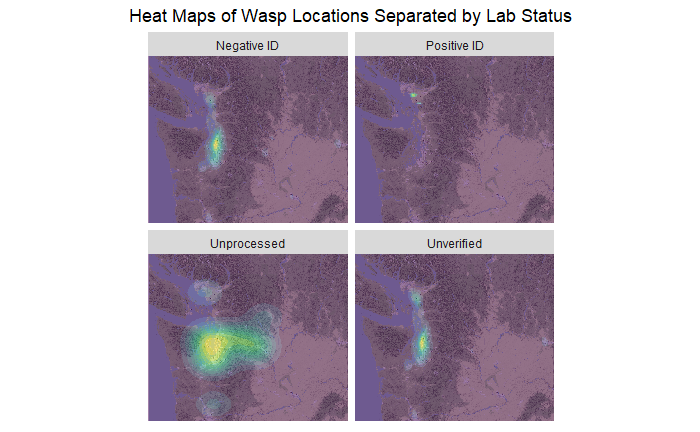
\includegraphics[width=0.6\textwidth]{images/facet_full.png}
    \caption{Heat Map Separated by Lab Type}
\end{figure}

It can be seen that all the positive results are located in the North-Western portion of Washington state, primarily in port regions. This is good news, as it shows that there has not been a lot of spread and there can be a focus on that one area. Next we can look at climate data in order to gain an insight as to where the hornet can potentially go that is suited to its needs.

\begin{figure}[H]
    \centering
    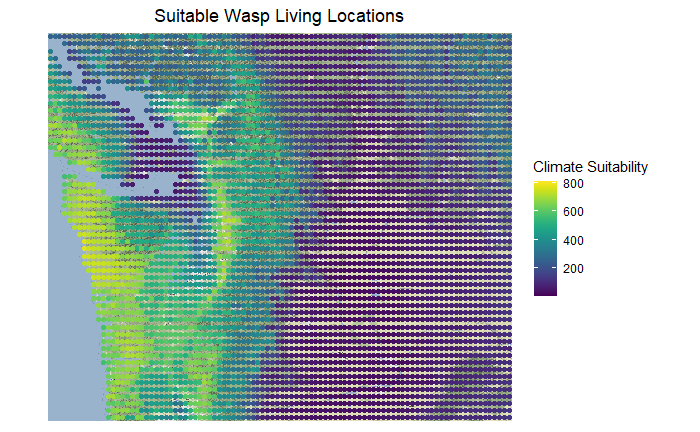
\includegraphics[width=0.6\textwidth]{images/weather.png}
    \caption{Plot of Climate Sustainability for hornets}
\end{figure}

It can be seen that only the coast of Washington has a high sustainability rating, everywhere else we will not need to worry about. Using these graphs will allow us to determine if the models make any sense using a common sense approach of looking at sustainability and seeing how far away from the initial location it is.

\section{Lat/Lon Model}

For this model we created a Gaussian Naive Bayes model and fed it the latitude, longitude and number of words in the notes. The word count ended up not mattering but the trained model managed to achieve 65.6\% accuracy which is impressive considering the amount of positive results.

\section{Image Classification Model}
In order to train our model for binary image classification, we used all the images provided to us in the dataset and sorted each image to its respective labels (excluding the videos), leaving unverified and unconfirmed data as sets for us to apply our model on to help predict future spread of the hornet. 

Additionally, due to the very limited amount of positive labeled images, we incorporated ten more images of the Asian wasp provided to us from Wikimedia Commons. Moreover, we applied image augmentation (like horizontal flip, vertical flip, rotation, blur, and etc) to help increase our training set using a Python tool from GitHub. With a 90, 10, 10 split for testing, training, and validation, we built our binary image classification model in R using the package Keras. 

\begin{figure}[H]
    \centering
    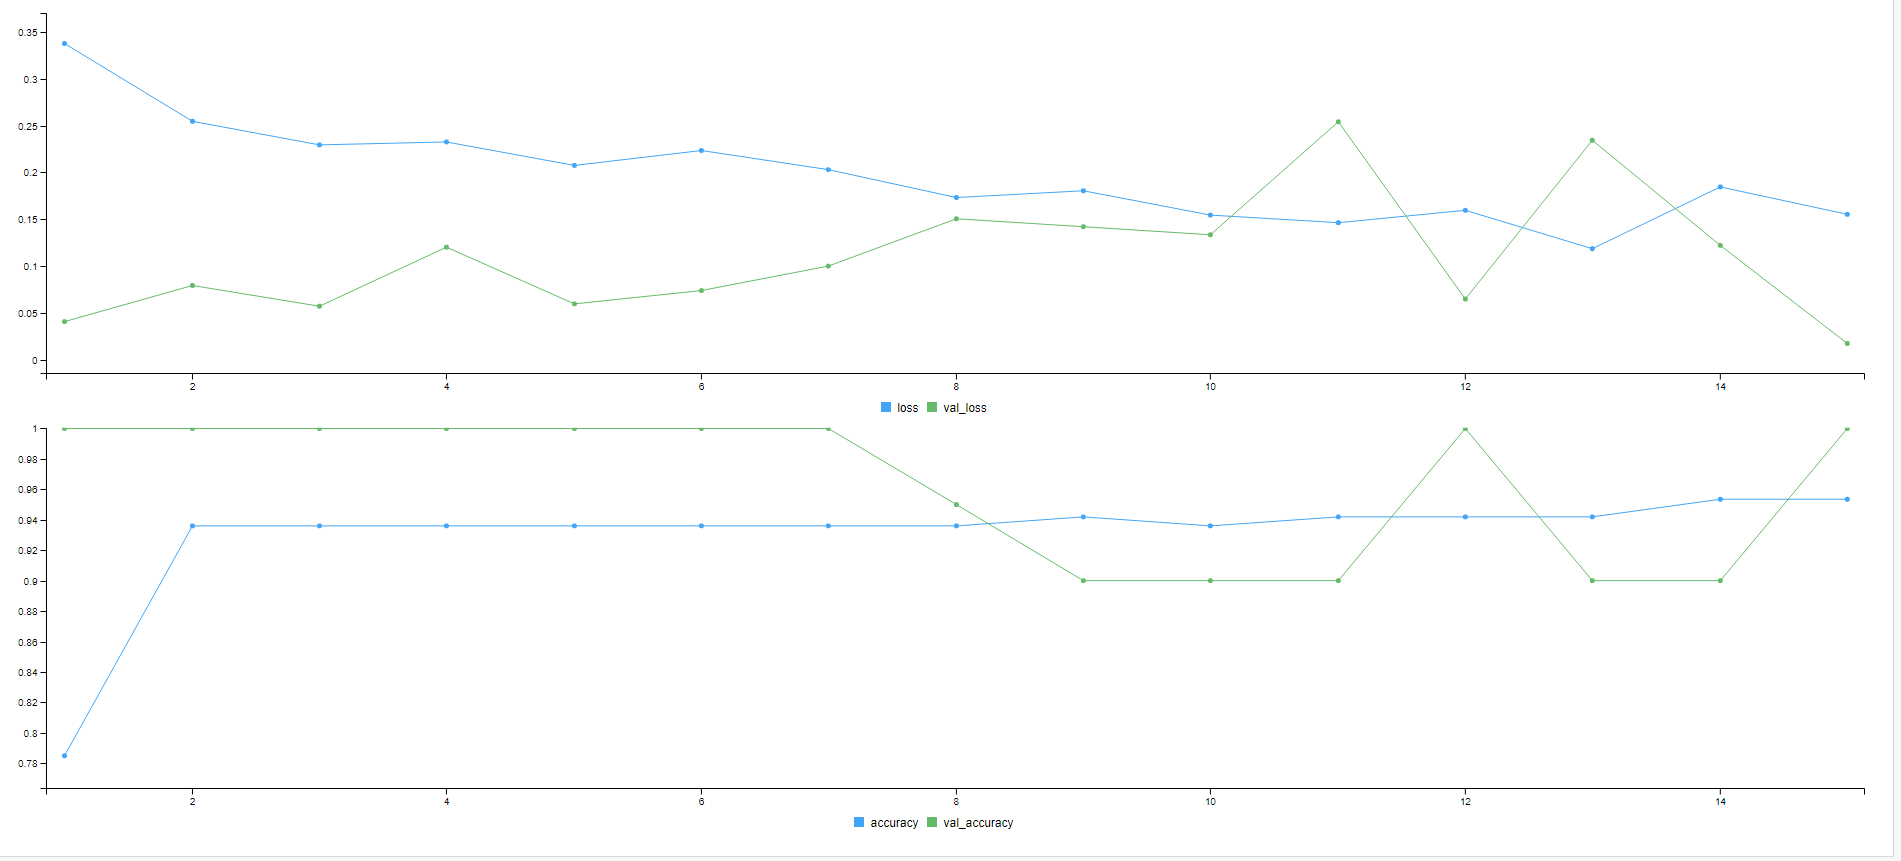
\includegraphics[width=0.6\textwidth]{images/trainingTestingPlot.png}
    \caption{Plot of Model 2 Accuracy and Loss}
\end{figure}


The metrics used to asses our model performance were loss and accuracy. The term "val loss" here refers to the validation loss and helped us optimize the hyperparamters of our neural networks (like the units per layer and how many layers we added). Accuracy is defined as the number of correct predictions over the total number of predictions; loss measures the prediction error (obtained from a loss function). Though our model had around 90\% percent accuracy on our training and validation sets, our model only correctly identifies new testing data about 50\% percent of the time (on average from several iterations). Applied to our unverified and unconfirmed datasets, the model only predicted one image as having a positive ID label (or as being the Vespa mandarinia).

\section{Frequency Analysis Model}

For this one we fed the notes into a fit multiclass model that was very inaccurate, topping 21\% for the highest accuracy. This demonstrates that using the notes given by people is not the wisest decision when trying to predict whether an observation had a hornet.

\section{Conclusions}
Ultimately, we must yield that without further investigation into a more accurate image classification model, investigation will still have to be carried out by the lab to identify reports as positive or negative. That the the Lat / Lon model had a decent level of success seems to suggest that there is a correlation between coordinates of sighting and its validity, meaning there is a region in which reports should be prioritized - a region we have yet identify. We have verified that there appears to be little to no correlation to word usage and frequency in the notes field and the ultimate ID of the report, going against our hypothesis that such an analysis would potentially be able to detect words that imply lack of confidence in their report. 


If we were provided more data, the image classification model would likely be better able to correctly idenitfy the wasp since our neural network would have more images to train on. One of the primary weakness of the neural network was the severely limited data it had to work with. Moreover, more correctly identified cases would help better balance our dataset (since the abnormal ratio of negative ids to positive ids resulted in a severely limited testing/training/validation set in order to ensure balance) and thus allow us to better map the unverified and unconfirmed data to help more effectively analyze the spread of the infestation.

\end{document}